\documentclass[11pt, oneside]{article}

%   ==============================================================================
%   This file is part of the 3D3A SABRE Toolkit.
%   
%   Joseph G. Tylka <josephgt@princeton.edu>
%   3D Audio and Applied Acoustics (3D3A) Laboratory
%   Princeton University, Princeton, New Jersey 08544, USA
%   
%   MIT License
%   
%   Copyright (c) 2017 Princeton University
%   
%   Permission is hereby granted, free of charge, to any person obtaining a copy
%   of this software and associated documentation files (the "Software"), to deal
%   in the Software without restriction, including without limitation the rights
%   to use, copy, modify, merge, publish, distribute, sublicense, and/or sell
%   copies of the Software, and to permit persons to whom the Software is
%   furnished to do so, subject to the following conditions:
%   
%   The above copyright notice and this permission notice shall be included in all
%   copies or substantial portions of the Software.
%   
%   THE SOFTWARE IS PROVIDED "AS IS", WITHOUT WARRANTY OF ANY KIND, EXPRESS OR
%   IMPLIED, INCLUDING BUT NOT LIMITED TO THE WARRANTIES OF MERCHANTABILITY,
%   FITNESS FOR A PARTICULAR PURPOSE AND NONINFRINGEMENT. IN NO EVENT SHALL THE
%   AUTHORS OR COPYRIGHT HOLDERS BE LIABLE FOR ANY CLAIM, DAMAGES OR OTHER
%   LIABILITY, WHETHER IN AN ACTION OF CONTRACT, TORT OR OTHERWISE, ARISING FROM,
%   OUT OF OR IN CONNECTION WITH THE SOFTWARE OR THE USE OR OTHER DEALINGS IN THE
%   SOFTWARE.
%   ==============================================================================

% Required packages
\usepackage[letterpaper, margin=1in, includeheadfoot]{geometry}
\usepackage{hyperref}
\usepackage{tabularx}

% Header and Footer
\usepackage{fancyhdr}
\pagestyle{fancy}
\renewcommand{\headrulewidth}{1pt}
\lhead{}\chead{\textsc{3D Audio and Applied Acoustics Laboratory $\cdot$ Princeton University}}\rhead{}
\lfoot{}\cfoot{\thepage}\rfoot{}

\renewcommand{\abstractname}{Summary} % Activate to modify the name of the Abstract
%\renewcommand*{\thefootnote}{\fnsymbol{footnote}} % Activate to use symbols rather than numbers for footnotes

% Additional packages
\usepackage{graphicx}
\usepackage{amssymb}
\usepackage{amsmath}
\usepackage[numbers,square,sort]{natbib}
\usepackage{tikz}

% User-defined commands
\newcommand{\citeref}[1]{Ref.~\cite{#1}}
\newcommand{\Citeref}[1]{Reference~\cite{#1}}
\newcommand{\citerefs}[1]{Refs.~\cite{#1}}
\newcommand{\Citerefs}[1]{References~\cite{#1}}
\newcommand{\figref}[1]{Fig.~\ref{#1}}
\newcommand{\Figref}[1]{Figure~\ref{#1}}
\newcommand{\figreftwo}[2]{Figs.~\ref{#1} and~\ref{#2}}
\newcommand{\eqnref}[1]{Eq.~(\ref{#1})}
\newcommand{\eqnreftwo}[2]{Eqs.~(\ref{#1}) and~(\ref{#2})}
\newcommand{\secref}[1]{Section~\ref{#1}}
\newcommand{\Secref}[1]{Section~\ref{#1}}
\newcommand{\secreftwo}[2]{Sections~\ref{#1} and~\ref{#2}}
\newcommand{\secrefthru}[2]{Sections~\ref{#1} through~\ref{#2}}
\newcommand{\tabref}[1]{Table~\ref{#1}}
\newcommand{\Tabref}[1]{Table~\ref{#1}}
\newcommand{\tabreftwo}[2]{Tables~\ref{#1} and~\ref{#2}}

\begin{document}

% Title and Author block
\begin{centering}
{\Large \textbf{SOFA/AmbiX Binaural Rendering (SABRE) Toolkit}}\\
\vspace{\baselineskip}
Joseph G.~Tylka\\
\href{mailto:josephgt@princeton.edu}{josephgt@princeton.edu}\\
\vspace{\baselineskip}
v0.11 -- October 26\textsuperscript{th}, 2017\\
\end{centering}

% Abstract
\begin{abstract}
The SOFA/ambiX binaural rendering (SABRE) toolkit is an open-source collection of MATLAB functions for generating custom binaural decoders for the ambiX binaural plug-in, which renders higher-order ambisonics to binaural.
This document describes the methods implemented in the toolkit and provides instructions for its use.
\end{abstract}

\section{Introduction}
This document is structured as follows.
In~\secref{sec:Conventions}, we describe the ambiX mathematical conventions and subsequently,
in~\secref{sec:Decoding}, we describe the ambisonics decoding approaches implemented in this toolkit.
Then, in~\secref{sec:HRTFs}, we discuss the various processing options that can be applied to the HRTFs.
This information was originally published by~\citet{TylkaChoueiri2017}, but may be updated here to reflect the current version of the toolkit.
Finally, in~\secref{sec:Functions}, we describe the various functions included in the toolkit and how to use them.

\subsection{Contents}
The toolkit consists of the following items:
\begin{enumerate}
\item the source \LaTeX~files for this manual (\texttt{/doc/});
\item some DSP-related MATLAB functions (\texttt{/dsp/});
\item a MATLAB file containing examples of how to use the toolkit (\texttt{/examples.m});
\item some MAT files containing spherical grids and corresponding quadrature weights (\texttt{/grids/});
\item some SOFA-formatted HRTFs (\texttt{/hrtfs/}); and
\item the core set of MATLAB functions for the toolkit (\texttt{/SABRE\_*.m}).
\end{enumerate}

%%%% Conventions %%%%
\section{Conventions}\label{sec:Conventions}
In accordance with the ambiX specification~\citep{Nachbar2011},
we use real-valued spherical harmonics as given by
\begin{equation*}
Y_l^m(\theta,\phi) = N_l^{|m|} P_l^{|m|} (\sin \theta) \times \left\{
    \begin{array}{cl}
	\cos m \phi & \textrm{for } m \geq 0,\\[8pt]
	\sin |m| \phi & \textrm{for } m < 0,
    \end{array}\right.
\end{equation*}
where $P_l^m$ is the associated Legendre polynomial of degree $l$ and order $m$,
as defined in the MATLAB \texttt{legendre} function by\footnote{See:~\url{https://www.mathworks.com/help/matlab/ref/legendre.html}}
\begin{equation*}
P_l^m(x) = (-1)^m (1 - x^2)^{m/2} \frac{d^m}{dx^m} P_l(x), 
\quad\quad \textrm{with} \quad\quad
P_l(x) = \frac{1}{2^l l!} \left[ \frac{d^l}{dx^l}(x^2 - 1)^l \right],
\end{equation*}
and $N_l^m$ is a normalization term which, for the Schmidt seminormalized (SN3D)
spherical harmonics with Condon-Shortley phase,\footnote{Note that including
Condon-Shortley phase in the normalization term cancels it in the associated Legendre term.}
is given by~\citep{Nachbar2011}
\begin{equation*}
N_l^m = (-1)^m \sqrt{\frac{2 - \delta_m}{4 \pi} \frac{(l-m)!}{(l+m)!}},
\end{equation*}
where $\delta_m$ is the Kronecker delta.
With an inner product defined by integrating over all directions, the squared-norm of these spherical harmonics is thus given by
\begin{equation*}
\left\| Y_l^m \right\|^2 = \frac{1}{2 l + 1}.
\end{equation*}

We also adopt the ambisonics channel numbering (ACN) convention~\citep{Nachbar2011}
such that for a spherical harmonic function of degree $l \in [0,\infty)$ and order $m \in [-l,l]$,
the ACN index $n$ is given by $n = l (l + 1) + m$ and we denote the spherical harmonic function by $Y_n \equiv Y_l^m$.

%%%% Decoding %%%%
\section{Decoding Ambisonics}\label{sec:Decoding}
Implemented in this toolkit are several basic methods of decoding ambisonics (described below),
but the Ambisonic Decoder Toolbox (ADT)\footnote{The ADT is available online at:~\url{https://bitbucket.org/ambidecodertoolbox/adt.git}} is a much more comprehensive tool for creating state-of-the-art ambisonic decoders~\citep{Heller2012}.
Consequently, one intended use of this toolkit is to add custom HRTFs to an existing ambiX decoder preset (such as those generated using the ADT).\footnote{At present, the SABRE toolkit is only compatible with single-band decoders. Consequently, multi-band decoders should be implemented in parallel (as a bank of single-band decoders), downstream of a crossover network.}
Note that doing so requires the user to specify the grid of speaker positions, as that information is not explicitly contained in ambiX decoder presets.

Generally, the decoding matrix, $\mathbf{D}$, determines the loudspeaker signals, $x_q$, given by
\begin{equation}
\mathbf{x} = 
\begin{bmatrix}
x_{1}(t) \\ x_{2}(t) \\ \vdots \\ x_{Q}(t)
\end{bmatrix}
 = \mathbf{D} \cdot 
\begin{bmatrix}
a_{0}(t) \\ a_{1}(t) \\ \vdots \\ a_{N-1}(t)
\end{bmatrix}
 = \mathbf{D} \cdot \mathbf{a},
\end{equation}
where $Q$ is the number of loudspeakers and $a_n$ is the ambisonic signal for ACN index $n$.
For a thorough review of ambisonic decoding theory and practice,
the reader is referred to the works of~\citet{Heller2008,Heller2012}.

Assuming a free field and ideal loudspeakers that are equidistant from the listener,
the resulting binaural pressure signals are given by
\begin{equation}
p^{\text{L,R}}(t) = \mathbf{h}^{\text{L,R}} \ast \mathbf{x}
 = \sum_{q=1}^Q h_{q}^{\text{L,R}}(t) \ast x_{q}(t),
\end{equation}
where `$\ast$' denotes convolution and
\begin{equation}
\mathbf{h}^{\text{L,R}} = 
\begin{bmatrix}
h_{1}^{\text{L,R}}(t) & h_{2}^{\text{L,R}}(t) & \cdots & h_{Q}^{\text{L,R}}(t)
\end{bmatrix}
\end{equation}
is a vector containing the head-related impulse responses (HRIRs) for a given listener
and for the directions of each loudspeaker.
The superscript ``$\text{L,R}$'' denotes the response at the left or right ear, respectively.

\subsection{Basic Decoding}
Following traditional ambisonic theory,
we consider the ambisonic signals produced at the center of the loudspeaker array
in response to the loudspeaker signals, given by
\begin{equation}
a_n(t) = \sum_{q=1}^{Q} Y_{n}(\hat{v}_q) x_q(t).
\end{equation}
Equivalently, in matrix form, we have $\mathbf{a} = \mathbf{Y} \cdot \mathbf{x}$, where
\begin{equation}\label{eq:YMatrix}
\mathbf{Y} = 
\begin{bmatrix}
Y_{0}(\hat{v}_1) & Y_{0}(\hat{v}_2) & \cdots & Y_{0}(\hat{v}_Q) \\
Y_{1}(\hat{v}_1) & Y_{1}(\hat{v}_2) & \cdots & Y_{1}(\hat{v}_Q) \\
\vdots & \vdots & \ddots & \vdots \\
Y_{N-1}(\hat{v}_1) & Y_{N-1}(\hat{v}_2) & \cdots & Y_{N-1}(\hat{v}_Q)
\end{bmatrix}.
\end{equation}
From this formulation, we obtain the basic (pseudoinverse) decoder, given by~\citep[Appendix~A.1]{Heller2008}
\begin{equation}\label{eq:PinvDecoder}
\mathbf{D} = \mathbf{Y}^{+},
\end{equation}
where $(\cdot)^{+}$ denotes pseudoinversion.

\subsection{Quadrature Decoding}
Given higher-order ambisonics signals, $a_n$, the so-called \textit{signature function}, $\mu$, in the direction $\hat{v}_q$ is given by~\citep{Duraiswami2005a}
\begin{equation}\label{eq:A2mu}
\mu(t,\hat{v}_q) = \sum_{n=0}^{N-1} a_n(t) \frac{Y_n(\hat{v}_q)}{\left\|Y_n\right\|^2}.
\end{equation}
Equivalently, in matrix form, we have
\begin{equation}
\begin{bmatrix}
\mu(t,\hat{v}_1) \\ \mu(t,\hat{v}_2) \\ \vdots \\ \mu(t,\hat{v}_Q)
\end{bmatrix} 
= \mathbf{Y}^{\textrm{T}} \cdot \mathbf{F}^{-1} \cdot \mathbf{a},
\end{equation}
where $Q$ is now the number of plane-wave terms and $\mathbf{F}$ is a diagonal matrix given by
\begin{equation}
\mathbf{F} = \text{diag} \left\{ \begin{bmatrix} \left\|Y_0\right\|^{2} & \left\|Y_1\right\|^{2} & \cdots & \left\|Y_{N-1}\right\|^{2} \end{bmatrix} \right\}.
\end{equation}

The signature function represents the coefficients of a plane-wave decomposition of the sound field,
such that the binaural pressure signals can be approximately reconstructed using a finite number of plane-waves, given by~\citep{Duraiswami2005a}
\begin{equation}
p^{\text{L,R}}(t) \approx \sum_{q=1}^Q h_{q}^{\text{L,R}}(t) \ast \left( w_q \mu(t,\hat{v}_q) \right)
 = \mathbf{h}^{\text{L,R}} \ast
\begin{bmatrix}
w_1 \mu(t,\hat{v}_1) \\ w_2 \mu(t,\hat{v}_2) \\ \vdots \\ w_Q \mu(t,\hat{v}_Q)
\end{bmatrix},
\end{equation}
where $w_q$ is the quadrature weight of the $q^\textrm{th}$ plane-wave term and is dependent on the chosen grid of directions.
Rearranging, we arrive at the quadrature decoder, given by
\begin{equation}
\mathbf{D} = 
\text{diag} \left\{ \begin{bmatrix} w_1 & w_2 & \cdots & w_Q \end{bmatrix} \right\}
\cdot \mathbf{Y}^{\textrm{T}} \cdot \mathbf{F}^{-1}.
\end{equation}

\subsection{Compact Decoding}
Now that we have established the typical decoding and binaural rendering signal chain,
we can derive an equally valid but more computationally efficient approach.
We first combine the HRIRs by performing the matrix multiplication with the decoder matrix,
which yields a vector of $N$ compacted HRIRs
\begin{equation}\label{eq:CompactHRTFs}
\mathbf{\tilde{h}}^{\text{L,R}} = 
\begin{bmatrix}
\tilde{h}_{0}^{\text{L,R}}(t) & \tilde{h}_{1}^{\text{L,R}}(t) & \cdots & \tilde{h}_{N-1}^{\text{L,R}}(t)
\end{bmatrix}
 = \mathbf{h}^{\text{L,R}} \cdot \mathbf{D}.
\end{equation}
This process simply combines the decoding matrix and per-direction HRIRs into a single set of filters.\footnote{Conceptually,
each compacted HRIR $\tilde{h}_{n}^{\text{L,R}}(t)$ represents the signals at the ears in response to an impulse sent through the $n^{\textrm{th}}$ HOA channel.}
The corresponding ``compact'' decoder is simply an $N \times N$ identity matrix, i.e., $\mathbf{\tilde{D}} = \mathbf{I}_{(N \times N)}$, such that $\mathbf{\tilde{h}}^{\text{L,R}} \cdot \mathbf{\tilde{D}} = \mathbf{h}^{\text{L,R}} \cdot \mathbf{D}$.
It's worth noting that, in the case of the basic pseudoinverse decoder, given by~\eqnref{eq:PinvDecoder},
the compacting process described by~\eqnref{eq:CompactHRTFs} is equivalent to to computing the
spherical-harmonics coefficients of the HRTFs, as done by~\citet[Sec.~IV]{RafaelyAvni2010}.

\subsection{Normalization}
For each HRIR (compacted or not), we first compute the maximum gain, $\alpha_q$, across the entire frequency response.
Subsequently, we attenuate each HRIR and amplify the corresponding row of the decoder matrix by that gain, i.e.,
\begin{equation}
\mathbf{\hat{h}}^{\text{L,R}} = \mathbf{h}^{\text{L,R}} \cdot \mathbf{G}^{-1},
\quad\quad
\text{and}
\quad\quad
\mathbf{\hat{D}} = \mathbf{G} \cdot \mathbf{D},
\end{equation}
where
\begin{equation}
\mathbf{G} = \text{diag} \left\{ \begin{bmatrix} \alpha_1 & \alpha_2 & \cdots & \alpha_Q \end{bmatrix} \right\},
\end{equation}
such that $\mathbf{\hat{h}}^{\text{L,R}} \cdot \mathbf{\hat{D}} = \mathbf{h}^{\text{L,R}} \cdot \mathbf{D}$.
Finally, we normalize the overall decoder matrix such that the maximum absolute value of any element in matrix is unity.

\section{HRTF Processing}\label{sec:HRTFs}
This toolkit requires HRTFs to be stored stored in SOFA format~\citep{AES69-2015}.
The HRTF files contain, among other things, the measured HRIRs and the grid of corresponding measurement positions.
Depending on the decoder used, the HRTFs may need to be interpolated,
and depending on the intended playback system (e.g., type of headphones), the HRTFs may need to be equalized.
Consequently, the SABRE toolkit contains several options for carrying out these processes.

\subsection{Interpolation}
When measured HRTFs are not available at the desired grid positions, interpolation is performed through one of the following methods.

\paragraph{Nearest Neighbor:} By default, we perform nearest-neighbor interpolation.
This is carried out by minimizing the $\ell^2$ norm (Euclidean distance) between the desired position
$\vec{v}_{q'}$ and each measurement position $\vec{u}_q$.

\paragraph{Time Domain:} Alternatively, we can perform weighted-average interpolation of the HRIRs for three different interpolation schemes:
natural neighbor, linear, and spherical-harmonic.\footnote{For spherical-harmonic interpolation, the interpolation weights are given as a matrix by $\mathbf{W} = \mathbf{Y}_Q^+ \mathbf{Y}_{Q'}$, where $\mathbf{Y}_Q$ is given by~\eqnref{eq:YMatrix} for all measurement positions and up to some maximum order (by default, $L = 4$), and $\mathbf{Y}_{Q'}$ is the same for all desired positions.}
Generally, for some function $f_q$ measured at positions $\vec{u}_q$, the interpolated values, $f'_{q'}$, for all desired positions $\vec{v}_{q'}$, are given by
\begin{equation}\label{eq:interpolation}
\begin{bmatrix} f'_1 & f'_2 & \cdots & f'_{Q'} \end{bmatrix} =
\begin{bmatrix} f_1 & f_2 & \cdots & f_{Q} \end{bmatrix} \cdot \mathbf{W},
\end{equation}
where each element, $w_{q,q'}$, of $\mathbf{W}$ is the interpolation weight from measurement position $\vec{u}_q$ to the desired position $\vec{v}_{q'}$.
Before interpolating, we first measure the onset delays, $\tau_q^\text{L,R}$, using a 10\% ($-20$~dB) threshold for each impulse response.
We then align all of the impulse responses such that their onsets coincide at the earliest onset, 
and separately store the relative delays, given by
\begin{equation}
d_q^\text{L,R} = \tau_q^\text{L,R} - \min \left( \min_q \tau_q^\text{L},~ \min_q \tau_q^\text{R} \right).
\end{equation}
Then we compute interpolation weights from each measurement position to each desired position and interpolate,
using~\eqnref{eq:interpolation}, the time-aligned impulse responses and the relative delays.
Finally, we introduce the interpolated time delays to each interpolated impulse response.

\paragraph{Frequency Domain:} We can also interpolate by first decomposing the HRTFs into magnitude spectra and time delays.
The magnitude spectra are given (in dB) by
\begin{equation}
M_q^\text{L,R}(f) = 10 \log_{10} \left( \left| H_q^\text{L,R}(f) \right|^2 \right),
\end{equation}
where $H$ denotes the Fourier transform of $h$.
We then interpolate the magnitude responses and time delays using~\eqnref{eq:interpolation}.
The interpolated magnitude responses are then converted into minimum-phase impulse responses,
and the interpolated onset delays are introduced to yield the final interpolated HRIRs.

\subsubsection{Interpolation Threshold}
Optionally, we may apply a threshold to determine which desired positions are close enough to a measurement position such that they do not require interpolation.
For each desired position, we find the nearest measurement position and compute the angular distance between the two, given by
\begin{equation}
\psi = \cos^{-1} \left( \frac{\vec{u}_q \cdot \vec{v}_{q'}}{\|\vec{u}_q\| \cdot \|\vec{v}_{q'}\|} \right),
\end{equation}
where $\| \cdot \|$ denotes the $\ell^2$ norm of a vector.
If this angular distance exceeds a user-specified threshold, then the selected interpolation method is carried out.
Otherwise, nearest-neighbor interpolation is used.

\subsection{Equalization}
For optimal binaural playback, one should use individually equalized headphones~\citep{ScharerLindau2009}.
As this may not always be possible, we provide several methods of equalization
so that the user may try to compensate for the equalization of the headphones.
We design the equalization filters using the full set of measured HRTFs
and apply them to the (possibly interpolated) HRTFs for the desired positions.

\paragraph{None:} By default, the HRTFs are not equalized.
This option should only be used if the playback headphones will be individually equalized on the user's ears.

\paragraph{Frontal:} For headphones that use frontal-incidence ``free-field'' equalization,
we can equalize all HRTFs by the HRTF pair nearest to $(\theta,\phi) = (0,0)$.
The transfer function of the regularized inverse filter is given by~\citep{Farina2007a}
\begin{equation}\label{eq:EQ_Filter}
Z(f) = \frac{H^\ast(f)}{H^\ast(f) H(f) + \beta(f)},
\end{equation}
where $(\cdot)^\ast$ denotes complex conjugation and $\beta$ is a frequency-dependent regularization function.
This function is defined by a set of parameters, which are defined graphically in~\figref{fig:beta}, and whose default values are given by
\begin{equation*}
\begin{array}{l l l}
\beta_0 = 10^{-4}, &f_{L0} = 50~\text{Hz}, &f_{H0} = 21~\text{kHz}, \\
\beta_1 = 10^{-2}, &f_{L1} = 20~\text{Hz}, &f_{H1} = 22~\text{kHz}.
\end{array}
\end{equation*}

% Plot of beta profile
\begin{figure}
\centering
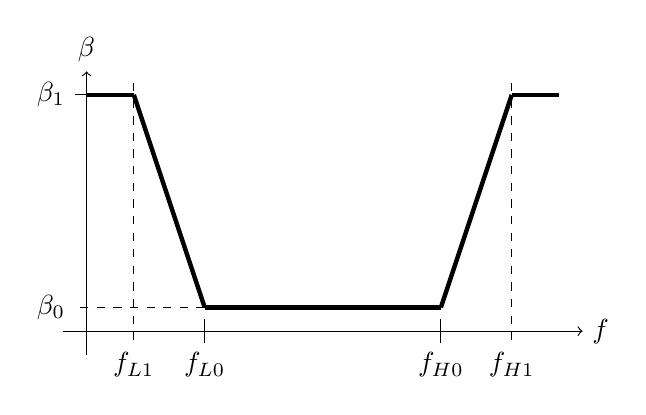
\begin{tikzpicture}[scale=3]
% Parameters
\def\betaone{1}; \def\betazero{0.1};
\def\fzero{0}; \def\fNyq{2};
\def\fLone{0.2}; \def\fLzero{0.5};
\def\fHzero{1.5}; \def\fHone{1.8};

% Axes
\draw[->] (\fzero-0.1,0) -- (\fNyq+0.1,0) node[right]{$f$};
\draw[->] (\fzero,-0.1) -- (\fzero,1.1) node[above]{$\beta$};

% Tick labels
\draw (\fzero+0.05,\betaone) -- (\fzero-0.05,\betaone) node[left]{$\beta_1$};
\draw[dashed] (\fLzero,\betazero) -- (\fzero-0.05,\betazero) node[left]{$\beta_0$};
\draw[dashed] (\fLone,\betaone+0.05) -- (\fLone,-0.05) node[below]{$f_{L1}$};
\draw (\fLzero,0.05) -- (\fLzero,-0.05) node[below]{$f_{L0}$};
\draw (\fHzero,0.05) -- (\fHzero,-0.05) node[below]{$f_{H0}$};
\draw[dashed] (\fHone,\betaone+0.05) -- (\fHone,-0.05) node[below]{$f_{H1}$};

% Plot
\draw[ultra thick] (\fzero,\betaone) -- (\fLone,\betaone);
\draw[ultra thick] (\fLone,\betaone) -- (\fLzero,\betazero);
\draw[ultra thick] (\fLzero,\betazero) -- (\fHzero,\betazero);
\draw[ultra thick] (\fHzero,\betazero) -- (\fHone,\betaone);
\draw[ultra thick] (\fHone,\betaone) -- (\fNyq,\betaone);
\end{tikzpicture}
\caption{Frequency-dependent regularization function of the inverse filters for HRTF equalization.}\label{fig:beta}
\end{figure}

\paragraph{Diffuse:} For headphones that employ diffuse-field equalization,
we can equalize the HRTFs by the average magnitude spectrum over all directions.
This is computed as the omnidirectional term of the spherical-harmonic decomposition of the HRTF magnitude spectra (in dB),
where the decomposition is computed using the pseudoinverse of $\mathbf{Y}$, given by~\eqnref{eq:YMatrix} for all measurement directions and up to order $L = 4$.
The equalization filter is then computed for the average magnitude spectrum using~\eqnref{eq:EQ_Filter}.

\paragraph{Horizontal:} Alternatively, we can compute an average HRTF over all horizontal-plane directions.
The procedure for this is very similar to the diffuse-field equalization, but the average spectrum is computed using only the HRTFs with elevation $|\theta| < 5^\circ$.
The equalization filter is then computed for the average magnitude spectrum using~\eqnref{eq:EQ_Filter}.

\section{MATLAB Functions}\label{sec:Functions}
The core MATLAB functions included in the toolkit are listed and described in~\tabref{tab:Functions}.

\begin{table}
\centering
  \begin{tabular}{| l | p{11cm} |}
    \hline
    \textbf{Function} & \textbf{Description} \\ \hline
    \texttt{SABRE\_AddHRTFDelays} & Introduces specified time delays into HRTF pairs;
    	returns the delayed HRIRs. \\ \hline
    \texttt{SABRE\_AmbiXPath} & Returns the ambiX binaural decoder preset directory. \\ \hline
    \texttt{SABRE\_BasicDecoder} & Designs a basic or quadrature ambisonics decoder up to a specified ambisonics order and for a specified grid of positions. \\ \hline
    \texttt{SABRE\_BinauralRenderer} & Creates and exports a custom ambiX binaural preset.
    	This is the primary function for using the toolkit; most other functions are called within this function. \\ \hline
    \texttt{SABRE\_EqualizationFilters} & Designs equalization filters for a set of HRTFs. \\ \hline
    \texttt{SABRE\_EqualizeHRTFs} & Applies equalization filters to a set of HRTFs. \\ \hline
    \texttt{SABRE\_GetDecoder} & Loads an existing or designs a new ambisonics decoder. \\ \hline
    \texttt{SABRE\_InterpolateHRTFs} & Interpolates measured HRTFs to a desired grid;
    	returns the interpolated HRTFs. \\ \hline
    \texttt{SABRE\_LoadGrid} & Loads a spherical grid and quadrature weights from a MAT file. \\ \hline
    \texttt{SABRE\_LoadHRTFs} & Loads HRTFs from a SOFA file;
    	returns the HRIRs, measurement grid, and sample rate. \\ \hline
    \texttt{SABRE\_NormalizeDecoder} & Normalizes BIRs and decoder gains. \\ \hline
    \texttt{SABRE\_ReadConfigFile} & Reads an ambiX binaural preset file;
    	returns the decoder matrix, HRTF filenames, and any global parameters specified in the file. \\ \hline
    \texttt{SABRE\_RemoveHRTFDelays} & Removes delays from HRTF pairs;
    	returns the time-aligned HRIRs and original delays. \\ \hline
    \texttt{SABRE\_RendererSettings} & Assembles inline binaural renderer settings into structs \texttt{config} and \texttt{flags}. \\ \hline
    \texttt{SABRE\_SphericalHarmonic} & Computes ambiX real-valued spherical harmonics;
    	returns a matrix of spherical harmonics up to a specified ambisonics order and for a specified grid of positions. \\ \hline
    \texttt{SABRE\_Start} & Starts the SABRE Toolkit and the SOFA API. \\ \hline
    \texttt{SABRE\_WriteConfigFile} & Writes an ambiX binaural preset file given the decoder matrix, HRTF filenames, and any global parameters. \\ \hline
    \end{tabular}
    \caption{Core MATLAB functions in the toolkit.}
    \label{tab:Functions}
\end{table}

\subsection{Creating a Binaural Renderer Configuration}
The function \texttt{SABRE\_BinauralRenderer} is the primary function used for creating a binaural renderer configuration,
and there are two ways to do this.
\paragraph{Option 1:} The direct method of creating a binaural renderer is to call \texttt{SABRE\_BinauralRenderer}, where the first 3 arguments must be
\begin{enumerate}
\item the output path,
\item the ambisonics order of the decoder, and
\item the SOFA file path,
\end{enumerate}
followed by any optional settings (see~\secref{sec:Options} below).
The corresponding MATLAB code for this might look like:
\begin{verbatim}
configFile = fullfile(SABRE_AmbiXPath,'3D3A-SABRE','example1.config');
maxOrder = 1;
sofaFile = fullfile('hrtfs','Subject2.sofa');
[config, flags] = SABRE_BinauralRenderer(configFile, maxOrder, sofaFile);
\end{verbatim}

\paragraph{Option 2:} An equivalent but less direct method is to first call \texttt{SABRE\_RendererSettings}.
This function takes as input a single cell array containing pairs of settings, and returns two structs,
\texttt{config} and \texttt{flags}, which are then passed directly to \texttt{SABRE\_BinauralRenderer}.
This approach may be more useful than the first when many options need to be specified.
The corresponding MATLAB code for this might look like:
\begin{verbatim}
temp = {'Output', configFile, 'Order', maxOrder, 'HRTF', sofaFile};
[config, flags] = SABRE_RendererSettings(temp);
[config, flags] = SABRE_BinauralRenderer(config, flags);
\end{verbatim}

\subsection{Renderer Settings}\label{sec:Options}
As discussed in previous sections, the toolkit implements a variety of methods and settings.
As alluded to in the previous section, there are two ways of specifying these options when creating the binaural renderer configuration.
All possible options are listed in~\tabref{tab:Options}.
\paragraph{Option 1:} The first method is to specify all of the desired options inline when creating the binaural renderer configuration.
In this case, after the first 3 required inputs, the options are listed as pairs, for example:
\begin{verbatim}
SABRE_BinauralRenderer(..., 'equalization', 'diffuse', 'sample rate', 48000);
\end{verbatim}
The options specified above would resample (if necessary) the HRTFs to 48~kHz and apply diffuse-field equalization.

\paragraph{Option 2:} The second method is to specify the options in the cell array of renderer settings.
In this case, the options are again listed as pairs, but may be given in any order. For example:
\begin{verbatim}
temp = {'equalization', 'diffuse', ..., 'sample rate', 48000};
[config, flags] = SABRE_RendererSettings(temp);
[config, flags] = SABRE_BinauralRenderer(config, flags);
\end{verbatim}
Note however that the 3 main settings (output path, decoder order, and SOFA file path) MUST be specified in the same cell array.

\begin{table}
\centering
	\begin{tabular}{| l | l | p{10cm} |}
	\hline
	\textbf{Option} & \textbf{Value} & \textbf{Description} \\ \hline
	\texttt{`output'} & \texttt{PATH} & Specify output file path for the ambiX .config file.
		NOTE: this input is mandatory. \\ \hline
	\texttt{`order'} & \texttt{L} & Specify the ambisonics order of the decoder.
		NOTE: this input is mandatory. \\ \hline
	\texttt{`hrtf'} & \texttt{PATH} & Specify the SOFA file path for the HRTFs.
		NOTE: this input is mandatory. \\ \hline
	\texttt{`grid'} & \texttt{R} & Use a custom speaker grid specified by \texttt{R}.
		\texttt{R} should be a $P \times 3$ matrix, where each row is a Cartesian vector.
		By default, the entire measurement grid in the SOFA file is used. \\ \hline
	\texttt{`method'} & \texttt{METHOD} & Specify the interpolation METHOD to be used.
		By default, nearest-neighbor interpolation is used. \\ \hline
	\texttt{`domain'} & \texttt{DOMAIN} & Specify the \texttt{DOMAIN} in which to interpolate.
		Must also specify an interpolation method. \\ \hline
	\texttt{`threshold'} & \texttt{THRESHOLD} & Specify the \texttt{THRESHOLD} for interpolation.
		If a measurement exists within \texttt{THRESHOLD} degrees from a desired position,
		then the nearest neighbor to that desired position is used. \\ \hline
	\texttt{`equalization'} & \texttt{TYPE} & Apply equalization of a given \texttt{TYPE} to the HRTFs.
		By default, no equalization is applied. \\ \hline
	\texttt{`sample rate'} & \texttt{Fs} & Specify desired HRTF sample rate for the decoder.
		By default, the sample rate of the HRTFs in the SOFA file is used for the decoder impulse responses. \\ \hline
	\texttt{`decoder'} & \texttt{PATH} & Load existing ambiX decoder.
		\texttt{PATH} should be the path to an existing ambiX .config file.
		NOTE: to use this option, you MUST also specify the corresponding grid. \\ \hline
	\texttt{`weights'} & \texttt{W} & Use quadrature-weighted decoder with weights \texttt{W}.
		\texttt{W} should be a length $P$ vector.
		NOTE: Weights are ignored if an existing ambiX decoder is used. \\ \hline
	\texttt{`compact'} & \texttt{X} & Compact the decoder into a square matrix.
		\texttt{X} should evaluate to either true or false. \\ \hline
	\texttt{`normalization'} & \texttt{X} & Normalize the decoder on a per-channel basis.
		\texttt{X} should evaluate to either true or false. \\ \hline
	\end{tabular}
	\caption{Options accepted by \texttt{SABRE\_BinauralRenderer} or \texttt{SABRE\_RendererSettings} to generate the \texttt{config} and \texttt{flags} structs.}
	\label{tab:Options}
\end{table}

%%TODO%% Add troubleshooting section

\section*{Acknowledgements}
This toolkit relies on the ambiX ambisonic plug-in suite\footnote{See:~\url{http://www.matthiaskronlachner.com/?p=2015}}
by M.~Kronlachner and requires head-related transfer functions (HRTFs) stored in the SOFA format.\footnote{See:~\url{https://www.sofaconventions.org}}
Accordingly, the SOFA API\footnote{See:~\url{https://github.com/sofacoustics/sofa}} for MATLAB is needed to import the HRTF files.

% References
\bibliographystyle{unsrtnat}
\bibliography{SABRE_Manual}

\end{document}